%% =====================================================================
%% Removing the Threshold: A Controlled Factorial Attribution of Decision
%% Rule and Region Grounding in Attribute Hallucination Detection
%%
%% Compile with pdfLaTeX (Overleaf default) or tectonic.  Every number that
%% depends on an experiment is either (a) copied from results/tables/*.csv
%% (AMBER, SHROOM-Vis) or (b) read from the macros/tables that
%% scripts/make_paper_tables.py writes into numbers.tex and tables/*.tex
%% from results/vaw/*.csv and results/calib/*.csv.  Nothing is typed by hand.
%% =====================================================================
\documentclass[11pt]{article}

\usepackage[margin=1in]{geometry}
\usepackage[T1]{fontenc}
\usepackage[utf8]{inputenc}
\usepackage{lmodern}
\usepackage{amsmath,amssymb,amsthm}
\usepackage{graphicx}
\usepackage{booktabs}
\usepackage{tabularx}
\usepackage{multirow}
\usepackage{makecell}
\usepackage{array}
\usepackage{xcolor}
\usepackage{caption}
\usepackage{subcaption}
\usepackage{enumitem}
\usepackage{pifont}
\usepackage{tikz}
\usetikzlibrary{positioning,arrows.meta,fit,calc,backgrounds}
\usepackage[section]{placeins}
\usepackage{url}
\usepackage[hidelinks]{hyperref}

\newcommand{\cmark}{\ding{51}}
\newcommand{\xmark}{\ding{55}}
\newcommand{\pmark}{$\circ$}
\newcommand{\yes}{\textsc{yes}}
\newcommand{\no}{\textsc{no}}
\newtheorem{proposition}{Proposition}
\captionsetup{font=small,labelfont=bf}
\setlist{itemsep=2pt,topsep=4pt}
\definecolor{modfill}{HTML}{EEF3FA}
\definecolor{modedge}{HTML}{3B5B8C}

\makeatletter
\newcommand{\tabinput}[1]{\@@input #1 }
\makeatother
% generated by scripts/make_paper_tables.py -- do not edit
\newcommand{\VAWdevAccA}{0.5620}
\newcommand{\VAWdevAccAp}{0.5513}
\newcommand{\VAWdevAccB}{0.7167}
\newcommand{\VAWdevAccC}{0.6113}
\newcommand{\VAWdevAccCalNullA}{0.5620}
\newcommand{\VAWdevAccCalNullC}{0.6113}
\newcommand{\VAWdevAccCalWordA}{0.6713}
\newcommand{\VAWdevAccCalWordC}{0.7010}
\newcommand{\VAWdevAccCp}{0.6007}
\newcommand{\VAWdevAccCstar}{0.6110}
\newcommand{\VAWdevAccD}{0.7767}
\newcommand{\VAWdevAccDext}{0.6989}
\newcommand{\VAWdevAccDstar}{0.7920}
\newcommand{\VAWdevAccFCnull}{0.5300}
\newcommand{\VAWdevAccWordPrior}{0.6070}
\newcommand{\VAWdevBminusA}{$+0.1547$}
\newcommand{\VAWdevBminusACI}{$[+0.1337,\,+0.1757]$}
\newcommand{\VAWdevBminusAp}{$+0.1653$}
\newcommand{\VAWdevBminusApCI}{$[+0.1440,\,+0.1867]$}
\newcommand{\VAWdevBminusCalNullA}{$+0.1547$}
\newcommand{\VAWdevBminusCalNullACI}{$[+0.1337,\,+0.1757]$}
\newcommand{\VAWdevCalNullAminusA}{$+0.0000$}
\newcommand{\VAWdevCalNullAminusACI}{$[+0.0000,\,+0.0000]$}
\newcommand{\VAWdevCalNullCminusC}{$+0.0000$}
\newcommand{\VAWdevCalNullCminusCCI}{$[+0.0000,\,+0.0000]$}
\newcommand{\VAWdevCalWordCminusC}{$+0.0897$}
\newcommand{\VAWdevCalWordCminusCCI}{$[+0.0743,\,+0.1050]$}
\newcommand{\VAWdevCalWordCminusWordPrior}{$+0.0940$}
\newcommand{\VAWdevCalWordCminusWordPriorCI}{$[+0.0767,\,+0.1120]$}
\newcommand{\VAWdevCminusA}{$+0.0493$}
\newcommand{\VAWdevCminusACI}{$[+0.0350,\,+0.0630]$}
\newcommand{\VAWdevCstarminusA}{$+0.0490$}
\newcommand{\VAWdevCstarminusACI}{$[+0.0343,\,+0.0633]$}
\newcommand{\VAWdevDextCoverage}{66.1\%}
\newcommand{\VAWdevDextminusAcov}{$+0.1402$}
\newcommand{\VAWdevDextminusAcovCI}{$[+0.1136,\,+0.1667]$}
\newcommand{\VAWdevDminusA}{$+0.2147$}
\newcommand{\VAWdevDminusACI}{$[+0.1933,\,+0.2360]$}
\newcommand{\VAWdevDminusB}{$+0.0600$}
\newcommand{\VAWdevDminusBCI}{$[+0.0367,\,+0.0827]$}
\newcommand{\VAWdevDminusC}{$+0.1653$}
\newcommand{\VAWdevDminusCCI}{$[+0.1453,\,+0.1853]$}
\newcommand{\VAWdevDminusCalNullC}{$+0.1653$}
\newcommand{\VAWdevDminusCalNullCCI}{$[+0.1453,\,+0.1853]$}
\newcommand{\VAWdevDminusCalWordC}{$+0.0757$}
\newcommand{\VAWdevDminusCalWordCCI}{$[+0.0523,\,+0.0993]$}
\newcommand{\VAWdevDminusFCnull}{$+0.2467$}
\newcommand{\VAWdevDminusFCnullCI}{$[+0.2147,\,+0.2787]$}
\newcommand{\VAWdevDminusWordPrior}{$+0.1697$}
\newcommand{\VAWdevDminusWordPriorCI}{$[+0.1430,\,+0.1967]$}
\newcommand{\VAWdevDstarminusCstar}{$+0.1810$}
\newcommand{\VAWdevDstarminusCstarCI}{$[+0.1617,\,+0.2010]$}
\newcommand{\VAWdevDstarminusD}{$+0.0153$}
\newcommand{\VAWdevDstarminusDCI}{$[-0.0020,\,+0.0333]$}
\newcommand{\VAWdevFallback}{6.2\%}
\newcommand{\VAWdevInteraction}{$+0.0107$}
\newcommand{\VAWgammaA}{0.00}
\newcommand{\VAWgammaC}{0.00}
\newcommand{\VAWnWordsC}{54}
\newcommand{\VAWtestAccA}{0.5797}
\newcommand{\VAWtestAccAp}{0.5800}
\newcommand{\VAWtestAccB}{0.7580}
\newcommand{\VAWtestAccC}{0.6087}
\newcommand{\VAWtestAccCalNullA}{0.5797}
\newcommand{\VAWtestAccCalNullC}{0.6087}
\newcommand{\VAWtestAccCalWordA}{0.5540}
\newcommand{\VAWtestAccCalWordC}{0.5833}
\newcommand{\VAWtestAccCp}{0.6120}
\newcommand{\VAWtestAccCstar}{0.6317}
\newcommand{\VAWtestAccD}{0.8133}
\newcommand{\VAWtestAccDext}{0.7269}
\newcommand{\VAWtestAccDstar}{0.8433}
\newcommand{\VAWtestAccFCnull}{0.5740}
\newcommand{\VAWtestAccWordPrior}{0.4913}
\newcommand{\VAWtestBminusA}{$+0.1783$}
\newcommand{\VAWtestBminusACI}{$[+0.1583,\,+0.1987]$}
\newcommand{\VAWtestBminusAp}{$+0.1780$}
\newcommand{\VAWtestBminusApCI}{$[+0.1577,\,+0.1987]$}
\newcommand{\VAWtestBminusCalNullA}{$+0.1783$}
\newcommand{\VAWtestBminusCalNullACI}{$[+0.1583,\,+0.1987]$}
\newcommand{\VAWtestCalNullAminusA}{$+0.0000$}
\newcommand{\VAWtestCalNullAminusACI}{$[+0.0000,\,+0.0000]$}
\newcommand{\VAWtestCalNullCminusC}{$+0.0000$}
\newcommand{\VAWtestCalNullCminusCCI}{$[+0.0000,\,+0.0000]$}
\newcommand{\VAWtestCalWordCminusC}{$-0.0253$}
\newcommand{\VAWtestCalWordCminusCCI}{$[-0.0417,\,-0.0090]$}
\newcommand{\VAWtestCalWordCminusWordPrior}{$+0.0920$}
\newcommand{\VAWtestCalWordCminusWordPriorCI}{$[+0.0747,\,+0.1093]$}
\newcommand{\VAWtestCminusA}{$+0.0290$}
\newcommand{\VAWtestCminusACI}{$[+0.0137,\,+0.0443]$}
\newcommand{\VAWtestCstarminusA}{$+0.0520$}
\newcommand{\VAWtestCstarminusACI}{$[+0.0367,\,+0.0677]$}
\newcommand{\VAWtestDextCoverage}{62.9\%}
\newcommand{\VAWtestDextminusAcov}{$+0.1585$}
\newcommand{\VAWtestDextminusAcovCI}{$[+0.1326,\,+0.1844]$}
\newcommand{\VAWtestDminusA}{$+0.2337$}
\newcommand{\VAWtestDminusACI}{$[+0.2133,\,+0.2533]$}
\newcommand{\VAWtestDminusB}{$+0.0553$}
\newcommand{\VAWtestDminusBCI}{$[+0.0333,\,+0.0767]$}
\newcommand{\VAWtestDminusC}{$+0.2047$}
\newcommand{\VAWtestDminusCCI}{$[+0.1857,\,+0.2233]$}
\newcommand{\VAWtestDminusCalNullC}{$+0.2047$}
\newcommand{\VAWtestDminusCalNullCCI}{$[+0.1857,\,+0.2233]$}
\newcommand{\VAWtestDminusCalWordC}{$+0.2300$}
\newcommand{\VAWtestDminusCalWordCCI}{$[+0.2063,\,+0.2533]$}
\newcommand{\VAWtestDminusFCnull}{$+0.2393$}
\newcommand{\VAWtestDminusFCnullCI}{$[+0.2073,\,+0.2713]$}
\newcommand{\VAWtestDminusWordPrior}{$+0.3220$}
\newcommand{\VAWtestDminusWordPriorCI}{$[+0.2967,\,+0.3473]$}
\newcommand{\VAWtestDstarminusCstar}{$+0.2117$}
\newcommand{\VAWtestDstarminusCstarCI}{$[+0.1933,\,+0.2297]$}
\newcommand{\VAWtestDstarminusD}{$+0.0300$}
\newcommand{\VAWtestDstarminusDCI}{$[+0.0133,\,+0.0473]$}
\newcommand{\VAWtestFallback}{8.0\%}
\newcommand{\VAWtestInteraction}{$+0.0263$}
\newcommand{\VAWtestObjects}{456}
\newcommand{\VAWtestShareFC}{76\%}
\newcommand{\VAWtestTriples}{1{,}201}
\newcommand{\VLMaccFC}{0.8864}
\newcommand{\VLMaccPrior}{0.5114}
\newcommand{\VLMaccThr}{0.8125}
\newcommand{\VLMdropped}{68}
\newcommand{\VLMfcCorrect}{88.6\%}
\newcommand{\VLMfcMinusThr}{$+0.0739$}
\newcommand{\VLMfcMinusThrCI}{$[+0.0057,\,+0.1364]$}
\newcommand{\VLMfprFC}{0.1136}
\newcommand{\VLMfprThr}{0.1023}
\newcommand{\VLMmodel}{claude-haiku-4-5-20251001}
\newcommand{\VLMpairCorrect}{64.8\%}
\newcommand{\VLMpairRev}{2.3\%}
\newcommand{\VLMpairSame}{33.0\%}
\newcommand{\VLMpairs}{88}
\newcommand{\VLMquestions}{176}
\newcommand{\VLMthrMinusPrior}{$+0.3011$}
\newcommand{\VLMthrMinusPriorCI}{$[+0.2443,\,+0.3580]$}
\newcommand{\VLMyesPrior}{0.0568}
\newcommand{\VLMyesThr}{0.4148}


\title{\textbf{Removing the Threshold: A Controlled Factorial Attribution of Decision Rule and Region Grounding in Attribute Hallucination Detection}}
\author{Vanuj Gangrade, Aryan Bhandari, Harsh Parmeshwaram, and Gautam Majumdar\\[6pt]
\normalsize School of Computer Science and Engineering, Vellore Institute of Technology,\\
\normalsize Vellore, Tamil Nadu, India}
\date{}

\begin{document}
\maketitle

\begin{abstract}
Vision--language models (VLMs) often hallucinate object attributes: they name an object correctly but ascribe to it a colour, material, state or action that the image does not show. Detectors for this error usually verify each claim \emph{independently}. A score for ``the jacket is leather'' is compared with a threshold, and recent work has shown that many resulting errors are threshold-placement errors, which can be reduced by calibrating the threshold (e.g.\ VISOR). Detectors also increasingly ground the claim in the image region of the named object, on the assumption that localisation is what makes verification reliable. This paper asks how much each design choice actually contributes. We do not calibrate the threshold. Instead, we remove the dependence on it by replacing independent threshold-based verification with \emph{pairwise forced-choice verification}: the claimed attribute is accepted only if it outscores a competing attribute on the same visual evidence. We then isolate the decision rule from region grounding in a controlled $2\times2$ factorial design (whole image or detected region, crossed with threshold or forced choice). The scorer (SigLIP), detector (OWLv2), prompts and data are held fixed, and contrasts are tested with an image-level paired bootstrap. On three datasets, AMBER, SHROOM-Vis and VAW (the benchmark on which VISOR's calibration analysis was performed), the relative decision rule explains most of the observed gain. On AMBER's held-out test split, forced choice alone adds $+0.2036$ accuracy (95\% CI $[+0.1781,+0.2288]$) of a combined $+0.2260$, against $+0.0201$ for region grounding alone. The corresponding figures on SHROOM-Vis are $+0.2235$ of $+0.2354$, and on VAW \VAWtestBminusA{} of \VAWtestDminusA{}. A pair-level analysis shows why: under a threshold, the scorer usually ranks the true attribute first, yet both attributes fall on the same side of the threshold in most pairs. Calibration applied to the same scorer does not close the gap to forced choice. VISOR-style null-image calibration leaves accuracy unchanged. Per-word thresholds approach forced choice only on AMBER, where an image-blind word prior alone reaches 0.7592, and they fail to transfer from development to test on VAW. A check with a generative multimodal LLM as the scorer, on colour attributes, reproduces the same pair-level failure mode but a much smaller gain ($+0.0739$), which is consistent with a better-calibrated verifier having less miscalibration to remove. The verifier uses 0.36B open-weight parameters, no language model and no training.
\end{abstract}

\noindent\textbf{Keywords:} multimodal hallucination detection; attribute hallucination; forced choice; threshold calibration; region grounding; factorial ablation; vision--language models

%% ---------------------------------------------------------------------
\section{Introduction}\label{sec:intro}
%% ---------------------------------------------------------------------

Large vision--language models (VLMs)~\cite{liu2023llava} describe images fluently but not always faithfully. This failure, \emph{multimodal hallucination}, is one of the most studied reliability problems of current VLMs~\cite{bai2024survey,chen2025survey}. Object hallucination, in which the model mentions an object that is not present, is measured by CHAIR~\cite{rohrbach2018chair} and POPE~\cite{li2023pope}. \emph{Attribute hallucination} is subtler: the object is present and correctly named, but a property ascribed to it, such as ``the frisbee is \emph{black}'' or ``the jacket is \emph{leather}'', is wrong~\cite{wang2023amber,zhang2026visor}. A detector cannot catch it by checking that the object exists. It must check a property of a particular object.

Post-hoc detectors verify each claim against the image, and most do so \emph{independently and absolutely}. A tool-based pipeline~\cite{yin2023woodpecker,jing2024faithscore,chen2024unihd,yang2026omnihallu} decomposes a response into atomic claims and asks a verifier whether each claim holds. A contrastive scorer~\cite{radford2021clip,zhai2023siglip,hessel2021clipscore} compares an image--text score with a threshold. A VLM probed with ``Is the jacket leather?'' answers \yes{} when $\mathrm{logit}(\yes)-\mathrm{logit}(\no)$ exceeds zero~\cite{zhang2026visor}. In every case the verdict depends on where an absolute decision boundary lies on an uncalibrated score.

Two lines of recent work address this weakness from different directions. The first treats the boundary as the problem and \emph{calibrates} it. VISOR~\cite{zhang2026visor} decomposes attribute yes/no probing on VAW~\cite{pham2021vaw} into a visual signal and a null-image language prior. It shows that colour and state false positives are mostly \emph{threshold-placement} errors, in which the visual signal points in the right direction with too small a margin, and it corrects them by shifting the decision boundary with a calibrated prior term. The same idea underlies contextual calibration of language models with content-free inputs~\cite{zhao2021calibrate,fei2023labelbias}, calibrated span fusion in the SHROOM-Visions shared task~\cite{abebe2026spancalib}, and calibration of zero-shot CLIP~\cite{levine2023clipcalib}. The second line treats \emph{evidence} as the problem and grounds the claim in the image. VBackChecker~\cite{guo2026vbackchecker} accepts a sentence only if a pixel-level grounding model can segment what it describes. Counterfactual grounding~\cite{song2026countervhd} contrasts the localisation of an entity with that of a perturbed entity. Region-level prompting~\cite{subramanian2022reclip,shtedritski2023redcircle} crops or marks the object before scoring it.

Both lines keep the same decision structure, an absolute verdict on a single claim. Calibration moves the threshold but keeps it, and the calibrated threshold must still be fitted on labelled data and must transfer to new images, objects and words. Grounding changes the evidence but leaves the decision rule as it was. VBackChecker emits a single accept/reject token, and the counterfactual detector of~\cite{song2026countervhd} merges its factual and counterfactual confidences into one uncertainty score that is thresholded. Because detectors are evaluated end to end, a reported improvement cannot be attributed to one change or the other. We found no prior work that measures, on the same scorer, prompts and data, how much of an improvement in attribute hallucination detection comes from region grounding and how much from the decision rule (Section~\ref{sec:gap}).

\paragraph{This work.} We take the alternative that calibration leaves open: we \emph{avoid} the threshold rather than calibrating it. Attribute claims have a natural competing hypothesis: a frisbee that is blue is not black, and a jacket that is denim is not leather. A \emph{forced-choice} verifier accepts the claimed attribute only if it scores higher than a competing attribute on the same visual evidence. Any additive offset in the score, whether image-level brightness, clutter, scorer bias or a global language prior, cancels in the comparison (Proposition~\ref{prop:offset}), so the decision has no free parameter to calibrate. This is the two-alternative forced-choice argument of signal detection theory~\cite{green1966sdt,macmillan2005detection}, applied to hallucination detection.

We then \textbf{experimentally isolate} the contribution of the decision rule from that of region grounding. A $2\times2$ factorial design crosses \{whole image, detected region\} with \{independent threshold, forced choice\}. Everything else is held fixed: the scorer (SigLIP~\cite{zhai2023siglip}), the detector (OWLv2~\cite{minderer2023owlv2}), the prompt template, the model revisions and the data. Contrasts are tested with an image-level paired bootstrap~\cite{efron1979bootstrap,field2007clustered}. We run the design on three datasets: AMBER~\cite{wang2023amber}, SHROOM-Vis (a second benchmark we built over the SHROOM-Visions images~\cite{vazquez2026shroomvisions}), and VAW~\cite{pham2021vaw}, the dataset on which VISOR established its calibration remedy. On VAW we also compare forced choice directly with VISOR-style calibration on the same scorer.

\paragraph{Contributions.} Our contribution is not a new model and not forced choice as such, which is the standard zero-shot decision of contrastive models~\cite{radford2021clip} and a standard evaluation protocol for compositionality~\cite{yuksekgonul2023bow,thrush2022winoground,hsieh2023sugarcrepe}. It is the controlled measurement of a design choice that the hallucination-detection literature has calibrated around but not removed:
\begin{enumerate}[leftmargin=*]
\item \textbf{Controlled factorial attribution.} With scorer, prompts and data held fixed, a $2\times2$ design separates the effect of region grounding from the effect of the decision rule. It shows that replacing independent threshold-based verification with pairwise forced-choice verification yields the dominant improvement in attribute hallucination detection, on three datasets (Section~\ref{sec:attribution}).
\item \textbf{Removing the threshold versus calibrating it.} On the same scorer, forced choice is compared with VISOR-style null-image calibration and with per-word calibrated thresholds, both fitted on development data. Neither calibrator closes the gap. Image-blind controls show that per-word thresholds partly learn which attribute words tend to be true rather than reading the image (Section~\ref{sec:calib}).
\item \textbf{Mechanism at pair level.} We quantify a failure mode that per-sample analyses only imply. Under a threshold, the true and false attribute of a pair usually receive the \emph{same} answer, although the same scores rank them correctly (Section~\ref{sec:mechanism}).
\item \textbf{Grounding, measured honestly.} Region grounding is real but small. On VAW, an oracle arm that crops to the annotated instance box separates detector error from the value of grounding itself (Section~\ref{sec:oracle}).
\item \textbf{Scorer generality, bounded.} A generative multimodal LLM probed the same way reproduces the pair-level failure mode on colour attributes but gains far less from forced choice, which bounds the claim rather than inflating it (Section~\ref{sec:vlm}).
\item \textbf{Protocol.} Thresholds are frozen before each test split is opened, and every control was declared before it was run. Claims that failed to replicate are reported as withdrawn, and three construction artifacts in AMBER are documented (Section~\ref{sec:controlsres}).
\end{enumerate}

The paper is organised as follows. Section~\ref{sec:related} reviews related work and states the research gap. Section~\ref{sec:method} formulates the problem and describes the verifier, the decision rules and the factorial design. Section~\ref{sec:data} describes the three datasets, Section~\ref{sec:setup} the experimental protocol, and Section~\ref{sec:results} the results, including comparisons with VISOR and other prior work. Sections~\ref{sec:discussion} and~\ref{sec:threats} discuss implications and limitations, and Section~\ref{sec:conclusion} concludes.

%% ---------------------------------------------------------------------
\section{Related Work}\label{sec:related}
%% ---------------------------------------------------------------------

\subsection{Benchmarks for multimodal hallucination}
CHAIR~\cite{rohrbach2018chair} and POPE~\cite{li2023pope} measure object hallucination, POPE as balanced yes/no polling. HallusionBench~\cite{guan2024hallusionbench}, MMHal-Bench~\cite{sun2024llavarlhf}, HaloQuest~\cite{wang2024haloquest} and M-HalDetect~\cite{gunjal2024mhaldetect} broaden the scope. AMBER~\cite{wang2023amber} is an LLM-free benchmark covering existence, attribute and relation hallucination; its attribute questions come in contrastive (true, false) pairs over the same image and object. Detector benchmarks have grown from MHaluBench (420 claim-level instances over two modalities)~\cite{chen2024unihd} to R$^2$-HalBench, which contains rich-context responses from 18 MLLMs~\cite{guo2026vbackchecker}, and to OmniHallu-Bench, with 10{,}000 human-verified samples over six cross-modal tasks~\cite{yang2026omnihallu}. The SHROOM shared tasks~\cite{mickus2024shroom,vazquez2025mushroom} reached the multimodal setting with SHROOM-Visions 2026~\cite{vazquez2026shroomvisions}, which scores character-level hallucination spans. VAW~\cite{pham2021vaw} is an attribute-recognition dataset over Visual Genome~\cite{krishna2017visualgenome} with explicitly labelled \emph{negative} attributes per instance. VISOR repurposes it as a yes/no attribute-hallucination probe~\cite{zhang2026visor}, and we use it in the same way.

\subsection{Hallucination detectors}
\textbf{Decompose--verify--aggregate.} Woodpecker~\cite{yin2023woodpecker}, FaithScore~\cite{jing2024faithscore} and UNIHD~\cite{chen2024unihd} decompose a response into claims and verify each with tools such as open-set detectors, VQA models and OCR. OmniHallu~\cite{yang2026omnihallu} extends this to image, video and audio, in both comprehension and generation. It verifies attribute claims with an ensemble of large MLLMs combined by majority vote and a GPT-class aggregator, and it reports module ablations of claim decomposition and voting. \textbf{Grounding-based.} VBackChecker~\cite{guo2026vbackchecker} fine-tunes a LISA-style~\cite{lai2024lisa} grounding LLM to emit a segmentation token for groundable sentences and a rejection token otherwise. Its ablation attributes 5.2 points to the grounding loss. Counterfactual grounding~\cite{song2026countervhd} grounds an entity and a perturbed counterpart and thresholds an uncertainty score that combines the two. RelCheck~\cite{patil2026relcheck} adds relational grounding for correction. \textbf{Internal-state and span-level.} HALP~\cite{kogilathota2026halp} and VisER~\cite{hasanebrahimi2026viser} read hallucination signals from VLM internals. The top SHROOM-Visions systems fine-tune 8B-scale VLMs for span labelling~\cite{vazquez2026shroomvisions}, and SpanCalib-VLM fuses a span tagger with a generative VLM through calibrated probabilities~\cite{abebe2026spancalib}. Self-consistency methods such as SelfCheckGPT~\cite{manakul2023selfcheckgpt} need no external verifier.

\subsection{Threshold placement and calibration}
An independent yes/no decision needs a criterion, and a mis-set criterion produces systematic errors. POPE documents a yes-bias in VLMs~\cite{li2023pope}. On R$^2$-HalBench, VBackChecker reports open-source MLLM detectors with negative-class accuracy near 99\% and positive-class accuracy near 1\%, which is the signature of a misplaced decision boundary~\cite{guo2026vbackchecker}. VISOR~\cite{zhang2026visor} is the most direct treatment for attributes. Across 10{,}791 negative VAW samples and three VLM families, the visual logit margin predicts false positives far better than a null-image prior. Colour and state errors are diagnosed as low-margin, threshold-correctable errors (``Mechanism A''), and the VISOR-Calib operator, $\mathbb{1}[\delta_{\mathrm{vis}}-\gamma\,\delta_{\mathrm{prior}}>0]$, reduces colour false-positive rates by 11--17 points. Material errors are diagnosed as low signal-to-noise and routed to abstention or per-word adapters. This null-image correction is the multimodal analogue of contextual calibration with a content-free input~\cite{zhao2021calibrate,fei2023labelbias}. Calibration of confidence, rather than of the decision, is studied for CLIP~\cite{levine2023clipcalib} and modern networks generally~\cite{guo2017calibration}, and calibration is a primary metric in SHROOM-Visions~\cite{vazquez2026shroomvisions,abebe2026spancalib}. In all of these the decision remains absolute: calibration changes \emph{where} the threshold is, not \emph{whether} one is needed.

\subsection{Relative decisions}
Relative decisions are long established outside hallucination detection. Zero-shot CLIP classifies by an argmax over class prompts~\cite{radford2021clip}. ARO~\cite{yuksekgonul2023bow}, Winoground~\cite{thrush2022winoground} and SugarCrepe~\cite{hsieh2023sugarcrepe} \emph{evaluate} compositional understanding by asking whether a model prefers the correct caption to a minimally perturbed one. ReCLIP~\cite{subramanian2022reclip} takes an argmax over candidate \emph{regions}. LLM-as-judge studies compare pairwise comparison with single-answer grading~\cite{zheng2023judging}. Psychophysics has long preferred two-alternative forced choice to yes/no designs, because the observer's criterion cancels in a comparison~\cite{green1966sdt,macmillan2005detection}. None of these works uses forced choice between competing attribute values as the decision rule of a hallucination detector, compares it with a threshold under a fixed scorer, or separates its effect from that of grounding.

\subsection{Research gap and positioning}\label{sec:gap}
Table~\ref{tab:gap} sets the present work against the prior work closest to it, aspect by aspect. Each entry was checked against the full text of the cited paper, and the supporting sections are listed in Appendix~\ref{app:evidence}. Table~\ref{tab:capability} gives a capability comparison in the style of~\cite{guo2026vbackchecker,yang2026omnihallu}. The gap is specific. (i) The threshold problem is known, and the established remedy is to calibrate the threshold. (ii) Grounding is widely used and sometimes ablated, but never crossed with the decision rule under a fixed scorer. (iii) No work quantifies at pair level that a threshold verifier ranks the attributes correctly yet labels both the same way. The more defensible novelty is therefore methodological. We avoid the threshold through forced-choice verification, and we isolate experimentally how much of the improvement comes from the decision rule and how much from region grounding.

\begin{table}[!htbp]
\centering
\caption{Research gap. Each prior work is assessed on the six aspects that distinguish this study, from the full text of the cited papers (evidence locations in Appendix~\ref{app:evidence}). \cmark: yes; \pmark: partly or related; \xmark: no.}
\label{tab:gap}
\small
\begin{tabularx}{\textwidth}{>{\raggedright\arraybackslash}p{4.3cm}*{6}{>{\centering\arraybackslash}X}}
\toprule
Aspect & \makecell{VISOR\\\cite{zhang2026visor}} & \makecell{VBack-\\Checker\\\cite{guo2026vbackchecker}} & \makecell{Omni-\\Hallu\\\cite{yang2026omnihallu}} & \makecell{Counter-\\factual\\\cite{song2026countervhd}} & \makecell{Span-\\Calib\\\cite{abebe2026spancalib}} & \makecell{\textbf{This}\\\textbf{work}} \\
\midrule
Recognises the threshold / calibration issue & \cmark & \pmark & \pmark & \cmark & \cmark & \cmark \\
Uses calibration as the remedy & \cmark & \xmark & \pmark & \xmark & \cmark & \xmark$^{a}$ \\
Explicit forced choice between competing attributes & \xmark & \xmark & \xmark & \pmark$^{b}$ & \xmark & \cmark \\
Separates grounding effect from decision-rule effect & \xmark$^{c}$ & \pmark$^{d}$ & \xmark$^{e}$ & \xmark & \xmark & \cmark \\
Threshold ranks correctly but labels both attributes alike (pair level) & \pmark$^{f}$ & \xmark & \xmark & \xmark & \xmark & \cmark \\
Region $\times$ decision rule under one protocol & \xmark & \xmark & \xmark & \xmark & \xmark & \cmark \\
\bottomrule
\end{tabularx}\\[3pt]
\parbox{\textwidth}{\footnotesize $^{a}$Calibration is implemented here as a \emph{baseline} on the same scorer (Section~\ref{sec:calib}). $^{b}$A counterfactual competitor is grounded, but the two confidences are merged into an uncertainty score decided by a threshold. $^{c}$No region grounding is used. $^{d}$The grounding loss is ablated, but grounding and the accept/reject token are trained jointly. $^{e}$Ablations remove claim decomposition and voting. $^{f}$``Directionally correct but low-margin'' visual signals are reported per sample and per word, not as pair outcomes.}
\end{table}

\begin{table}[!htbp]
\centering
\caption{Capability comparison with representative detectors, as reported by their authors.}
\label{tab:capability}
\footnotesize
\setlength{\tabcolsep}{3pt}
\begin{tabularx}{\textwidth}{>{\raggedright\arraybackslash}p{2.9cm}*{6}{>{\centering\arraybackslash}X}}
\toprule
 & \makecell{UNIHD\\\cite{chen2024unihd}} & \makecell{Omni-\\Hallu\\\cite{yang2026omnihallu}} & \makecell{VBack-\\Checker\\\cite{guo2026vbackchecker}} & \makecell{VISOR\\\cite{zhang2026visor}} & \makecell{SHROOM-V.\\top-5\\\cite{vazquez2026shroomvisions}} & \makecell{\textbf{This}\\\textbf{work}} \\
\midrule
No LLM/MLLM in the verification loop & \xmark & \xmark & \xmark & \xmark & \xmark & \cmark \\
No task-specific training & \cmark & \pmark & \xmark & \pmark$^{\dagger}$ & \xmark & \cmark \\
Object-region evidence & \pmark & \pmark & \cmark & \xmark & \xmark & \cmark \\
Decision without a fitted threshold & \xmark & \xmark & \pmark & \xmark & \xmark & \cmark \\
Component contributions isolated & \xmark & \pmark & \pmark & \pmark & \xmark & \cmark \\
Evaluated on more than one dataset & \cmark & \cmark & \cmark & \pmark & \xmark & \cmark \\
Parameters in the verifier & GPT-4V & $>$70B & 7B & 3--7B & 8B & 0.36B \\
Output granularity & claim & claim & sentence & yes/no & span & claim \\
\bottomrule
\end{tabularx}\\[3pt]
\parbox{\textwidth}{\footnotesize $^{\dagger}$VISOR-Calib and VISOR-Abstain are training-free; VISOR-Adapt trains per-word LoRA adapters.}
\end{table}

%% ---------------------------------------------------------------------
\section{Method}\label{sec:method}
%% ---------------------------------------------------------------------

\subsection{Problem formulation}
Let $I$ be an image, and let a claim assert that object $o$ has attribute $a$, for example a colour, material, state or action. The verifier outputs $\hat y\in\{\yes,\no\}$, stating whether $I$ supports the claim. Attribute questions are evaluated as \emph{contrastive pairs}
\begin{equation}
p=(I,\,o,\,a^{+},\,a^{-}),
\label{eq:pair}
\end{equation}
where $a^{+}$ is true of $o$ in $I$ (gold \yes) and $a^{-}$ is a mutually exclusive alternative of the same kind that is false (gold \no). Each pair contributes two questions, ``Is the $o$ $a^{+}$?'' and ``Is the $o$ $a^{-}$?''. A false claim is a \emph{hallucinated} claim, so detecting hallucination means answering \no{} to $a^{-}$ while answering \yes{} to $a^{+}$. In AMBER the pair is supplied by the benchmark. In VAW both attributes come from human labels of the same instance: $a^{+}$ from its positive attributes and $a^{-}$ from its explicitly negative attributes. Section~\ref{sec:dext} removes the dataset-supplied competitor altogether.

\subsection{Verifier pipeline}
The verifier has six modules (Fig.~\ref{fig:flow}). \textbf{M1} parses a claim or benchmark question into the record of Eq.~\eqref{eq:pair}. \textbf{M2} localises $o$ with OWLv2~\cite{minderer2023owlv2} (\texttt{owlv2-base-patch16-ensemble}, 155M parameters), prompted with ``a photo of a $\{o\}$''. Boxes scoring below $\delta=0.10$ are discarded and duplicates removed by NMS at IoU $0.5$~\cite{neubeck2006nms}. \textbf{M3} pads the top box by $\rho=10\%$ per side, enforces a $64$\,px minimum and clips it to the image. If nothing is detected it falls back to the whole image and flags the record. \textbf{M4} scores the prompt $\pi(a,o)=$ ``a photo of a $\{a\}$ $\{o\}$'' against the region $R$ with SigLIP~\cite{zhai2023siglip} (\texttt{siglip-base-patch16-224}, 203M parameters):
\begin{equation}
s(R,a)=t\,\langle f_{\mathrm{img}}(R),\,f_{\mathrm{txt}}(\pi(a,o))\rangle+\beta,
\label{eq:siglip}
\end{equation}
on the raw logit scale. Each prompt is encoded independently, so no candidate can observe another. \textbf{M5} turns scores into answers using one of the decision rules below. \textbf{M6} computes metrics and paired contrasts. The constants $\delta,\rho$, the minimum crop size, the prompt template and both model revisions were fixed before the first experiment and are byte-identical across all three datasets. No constant was tuned.

\begin{figure}[!htbp]
\centering
\resizebox{\textwidth}{!}{%
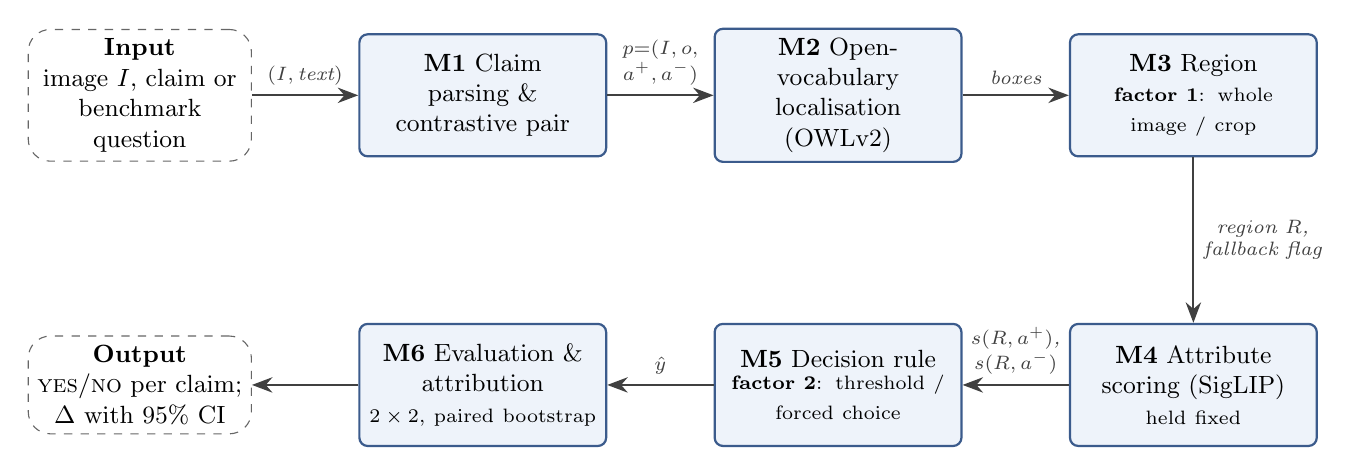
\begin{tikzpicture}[
  font=\small,
  mod/.style={draw=modedge, fill=modfill, rounded corners=3pt, line width=0.8pt, align=center, minimum height=1.55cm, text width=2.9cm},
  io/.style={draw=black!60, fill=white, rounded corners=8pt, align=center, minimum height=1.2cm, text width=2.6cm, dashed},
  lab/.style={font=\scriptsize\itshape, align=center, text=black!75},
  arr/.style={-{Stealth[length=2.6mm]}, line width=0.8pt, draw=black!75}]
\node[io] (in) {\textbf{Input}\\ image $I$, claim or\\ benchmark question};
\node[mod, right=1.35cm of in] (m1) {\textbf{M1} Claim parsing \&\\ contrastive pair};
\node[mod, right=1.35cm of m1] (m2) {\textbf{M2} Open-vocabulary\\ localisation\\ (OWLv2)};
\node[mod, right=1.35cm of m2] (m3) {\textbf{M3} Region\\ \scriptsize \textbf{factor 1}: whole image / crop};
\node[mod, below=2.1cm of m3] (m4) {\textbf{M4} Attribute\\ scoring (SigLIP)\\ \scriptsize held fixed};
\node[mod, left=1.35cm of m4] (m5) {\textbf{M5} Decision rule\\ \scriptsize \textbf{factor 2}: threshold /\\ \scriptsize forced choice};
\node[mod, left=1.35cm of m5] (m6) {\textbf{M6} Evaluation \&\\ attribution\\ \scriptsize $2\times2$, paired bootstrap};
\node[io, left=1.35cm of m6] (out) {\textbf{Output}\\ \yes/\no{} per claim;\\ $\Delta$ with 95\% CI};
\draw[arr] (in) -- node[lab, above]{$(I,\text{text})$} (m1);
\draw[arr] (m1) -- node[lab, above]{$p{=}(I,o,$\\$a^{+},a^{-})$} (m2);
\draw[arr] (m2) -- node[lab, above]{boxes} (m3);
\draw[arr] (m3) -- node[lab, right]{region $R$,\\ fallback flag} (m4);
\draw[arr] (m4) -- node[lab, above]{$s(R,a^{+})$,\\ $s(R,a^{-})$} (m5);
\draw[arr] (m5) -- node[lab, above]{$\hat y$} (m6);
\draw[arr] (m6) -- (out);
\end{tikzpicture}}
\caption{The verifier. The two factors of the study are the region switch in M3 and the decision switch in M5. The scorer, detector, prompt template, model revisions and data are identical in every cell.}
\label{fig:flow}
\end{figure}

\subsection{Decision rules}\label{sec:decision}
\textbf{Independent threshold.} Each question is answered alone:
\begin{equation}
\hat y(q)=\yes \iff s(R,a)\ge\tau .
\label{eq:threshold}
\end{equation}
The threshold $\tau$ is fitted by an exhaustive sweep that maximises development accuracy, frozen, and applied unchanged to the test split. This is the standard design of contrastive verifiers~\cite{hessel2021clipscore}, and it has the same structure as yes/no probing of a VLM, where $\delta_{\mathrm{vis}}\ge 0$ plays the role of $s\ge\tau$~\cite{zhang2026visor}.

\textbf{Pairwise forced choice.} The two candidates are compared on the same region:
\begin{equation}
\hat a=\arg\max_{a\in\{a^{+},a^{-}\}} s(R,a),\qquad \hat y(q^{\pm})=\yes \iff a^{\pm}=\hat a .
\label{eq:fc}
\end{equation}
Candidates are processed in alphabetical order, which carries no information about which one is true. Exact ties are counted, and none occurred. Forced choice has \emph{no free parameter}: nothing is fitted on any split.

\textbf{Why removing the threshold helps.} Write each score as an image-level offset plus an attribute-specific term, $s(R,a)=c(R,o)+g(R,a)$. The offset $c$ absorbs everything that shifts both prompts for the same region together: the learned bias $\beta$, brightness and clutter, the typicality of the object, crop scale, and any global language prior.

\begin{proposition}\label{prop:offset}
The forced-choice decision~\eqref{eq:fc} depends only on $g(R,a^{+})-g(R,a^{-})$ and is invariant to $c(R,o)$. The threshold decision~\eqref{eq:threshold} gives $q^{+}$ and $q^{-}$ the same answer whenever $c(R,o)$ places both scores on the same side of $\tau$, whatever their order. A calibrated threshold $\tau(w)$ or a prior-corrected score $s-\gamma s_{\varnothing}$ removes $c$ only to the extent that $c$ is constant within the calibration unit (a word, or the null-image prior).
\end{proposition}
\noindent\emph{Proof.} $s(R,a^{+})-s(R,a^{-})=g(R,a^{+})-g(R,a^{-})$, so the argmax is unchanged by any $c$. Under Eq.~\eqref{eq:threshold}, if $\min_a s\ge\tau$ both answers are \yes, and if $\max_a s<\tau$ both are \no; either way the pair has exactly one error. A calibration term that does not depend on $R$ cannot track a component of $c(R,o)$ that varies from image to image. $\square$

The proposition yields a testable prediction. If image-level offsets vary, threshold errors should be dominated by \emph{same-answer} pairs (both \yes{} or both \no) rather than by reversed pairs, and calibration should help only as far as the offset is shared within a word.

\subsection{Calibration baselines}\label{sec:calibdef}
To compare removing the threshold with calibrating it, two calibrators are applied to the \emph{same} scorer and regions. Both are fitted on development data only.
\begin{itemize}[leftmargin=*]
\item \textbf{Cal-null (VISOR-style).} Following VISOR-Calib~\cite{zhang2026visor} and contextual calibration~\cite{zhao2021calibrate}, the score is corrected by its value on a content-free null image $I_{\varnothing}$, a uniform grey $128\times128$ image as in VISOR:
\begin{equation}
\hat y(q)=\yes \iff s(R,a)-\gamma\, s(I_{\varnothing},a)\ \ge\ \tau ,
\label{eq:calnull}
\end{equation}
with $\gamma\in\{0,0.05,\dots,2\}$ and $\tau$ chosen jointly to maximise development accuracy.
\item \textbf{Cal-word.} A separate threshold $\tau_w$ for every attribute word $w$ with at least 10 development questions, and the global $\tau$ otherwise. This is the most flexible threshold calibration the data supports.
\end{itemize}

\subsection{The factorial design}
Crossing the two factors gives four cells (Table~\ref{tab:design}). A is the conventional baseline (whole image, threshold) and D the proposed verifier (detected region, forced choice). For cells $X,Y$ evaluated on the same questions $Q$, $\Delta_{X-Y}=\mathrm{Acc}_X(Q)-\mathrm{Acc}_Y(Q)$. B$-$A isolates the decision rule on the whole image, C$-$A isolates region grounding under a threshold, D$-$B isolates grounding given forced choice, D$-$A is the combined effect, and
\begin{equation}
\Delta_{\mathrm{int}}=\Delta_{D-C}-\Delta_{B-A}
\label{eq:interaction}
\end{equation}
measures interaction. Uncertainty is estimated with a paired cluster bootstrap whose resampling unit is the \emph{image}~\cite{efron1979bootstrap,field2007clustered}, with $B=10{,}000$ resamples and seed 20260907. The same resampled images are used for both cells, and the 95\% interval is the 2.5--97.5 percentile range. A contrast is called non-zero only if its interval excludes zero.

\begin{table}[!htbp]
\centering
\caption{The $2\times2$ design. Only the region and the decision rule differ between cells.}
\label{tab:design}
\small
\begin{tabular}{lcc}
\toprule
 & \textbf{Independent threshold} (Eq.~\ref{eq:threshold}) & \textbf{Forced choice} (Eq.~\ref{eq:fc}) \\
\midrule
\textbf{Whole image} ($R=I$) & A (baseline) & B \\
\textbf{Detected region} ($R=I[\tilde b]$) & C & D (proposed) \\
\bottomrule
\end{tabular}
\end{table}

\subsection{Controls}\label{sec:dext}
Every control was declared before it was run; the declarations are logged with the code.
\textbf{Base-rate-matched thresholds (A$'$, C$'$).} Forced choice emits exactly one \yes{} per pair, so on balanced data it receives the correct 50/50 answer distribution for free. A$'$ and C$'$ give the threshold cells the same information by setting $\tau$ so that the number of predicted \yes{} answers on development data equals the number of gold \yes{} answers.
\textbf{External competitor (D-ext).} D-ext removes the dataset-supplied competitor. Each question is answered alone, against the antonym of its attribute taken from a fixed map $\mathcal{M}$ (210 entries, committed before any D-ext result existed and unchanged for every dataset): $\hat y(q)=\yes\iff s(R,a)>s(R,\mathcal{M}(a))$. A D-ext verifier can answer \yes{} or \no{} to both questions of a pair. Unmapped questions are excluded, and coverage is reported.
\textbf{Oracle region (C$^{\ast}$, D$^{\ast}$; VAW only).} These crop to the human-annotated instance box instead of the OWLv2 box, with identical padding. They separate detector error from the value of grounding.
\textbf{Image-blind diagnostics.} \emph{WordPrior} answers each question with the majority development label of its attribute word and never opens an image. \emph{FC-null} applies forced choice to the null image $I_{\varnothing}$ and measures the scorer's text-only preference between the two words. \emph{Position-only} answers \yes{} to the lower question id and measures an AMBER construction artifact (Section~\ref{sec:artifacts}).

%% ---------------------------------------------------------------------
\section{Datasets}\label{sec:data}
%% ---------------------------------------------------------------------
Three datasets are used (Table~\ref{tab:datastats}). They differ in source, annotation process and vocabulary, and the claims of this paper are \emph{contrasts between cells measured on the same questions} within each dataset, never comparisons of absolute accuracy across datasets.

\textbf{AMBER}~\cite{wang2023amber}, human-annotated, 1{,}004 images. We use its state and action attribute questions, which M1 parses at a 100\% rate into 2{,}774 contrastive pairs (5{,}548 questions). The 2{,}072 number questions test counting and are excluded. Images were split 70/30 into development and test with seed 20260907, frozen on first write. The method was developed on AMBER, and its test split was opened once.

\textbf{SHROOM-Vis}, silver-standard, built by us over the images of SHROOM-Visions 2026~\cite{vazquez2026shroomvisions} (drawn from HaloQuest~\cite{wang2024haloquest} and VISaGE). It contains 900 images annotated in AMBER's schema by a VLM (Claude Opus~5) that is neither of the models under test, under an annotation policy frozen before any result existed. The policy requires same-dimension, mutually exclusive, image-dependent negatives, and drops a pair rather than guess. 898 images are usable, giving 2{,}523 pairs; 32.9\% of pairs involve objects outside AMBER's vocabulary. AMBER's id-ordering artifact is deliberately not reproduced. The labels have no human verification pass, and the dataset is reported as silver-standard throughout.

\textbf{VAW}~\cite{pham2021vaw}, human-annotated, over Visual Genome images~\cite{krishna2017visualgenome}. VAW labels each object instance with positive attributes and \emph{explicit negative attributes}. Following VISOR~\cite{zhang2026visor}, we use the \emph{color} (61 words), \emph{material} (52) and \emph{state} (11) attribute types from VAW's type file. A pair is formed for an instance and a type when both a positive and a negative attribute of that type exist. One of each is drawn with a seeded generator, so both questions of every pair come from human labels. We keep instances whose box is at least 20\,px on each side and whose object name is the only annotated instance of that name in the image, a partial guard against referential ambiguity. At most one pair is taken per image. The test split draws 1{,}500 pairs (600 color, 500 material, 400 state) from VAW's test set. The development split draws the same quotas from VAW's validation set, completed from its training set where validation is too small; the two splits share no image. The protocol was written and frozen before any model was run on VAW.

\begin{table}[!htbp]
\centering
\caption{Dataset statistics. Pairs are contrastive (true, false) attribute pairs on the same image and object; each contributes two questions. All three are exactly balanced at pair level.}
\label{tab:datastats}
\small
\begin{tabular}{lrrr}
\toprule
 & \textbf{AMBER} & \textbf{SHROOM-Vis} & \textbf{VAW} \\
\midrule
Labels & human & VLM (silver) & human \\
Attribute types & state, action & state, action & color, material, state \\
Competitor source & benchmark pair & frozen policy & human negative label \\
Dev: questions / images & 3{,}858 / 696 & 3{,}534 / 628 & 3{,}000 / 1{,}500 \\
Test: questions / images & 1{,}690 / 296 & 1{,}512 / 270 & 3{,}000 / 1{,}500 \\
Distinct objects (test) & --- & --- & \VAWtestObjects \\
Distinct (object, $a^{+}$, $a^{-}$) triples (test) & 352 & 462 & \VAWtestTriples \\
Detector fallback rate (test) & 4.6\% & 3.3\% & \VAWtestFallback \\
\bottomrule
\end{tabular}
\end{table}

%% ---------------------------------------------------------------------
\section{Experimental Setup}\label{sec:setup}
%% ---------------------------------------------------------------------
\textbf{Protocol.} Every fitted quantity ($\tau$ for A, C, C$^{\ast}$, A$'$, C$'$; $(\gamma,\tau)$ for Cal-null; $\tau_w$ for Cal-word; the WordPrior table) is fitted on the development split and frozen. Each test split was opened once, after development work on that dataset was complete. Development numbers fit $\tau$ on the evaluated data, which favours the threshold cells, so development comparisons are conservative. Test numbers are the headline results. The calibration baselines and image-blind diagnostics were declared in advance for VAW. For AMBER and SHROOM-Vis they were added after the test splits had been opened (Section~\ref{sec:calib}). They are baselines, not modifications of the proposed method, and they are labelled as post-hoc wherever they appear.

\textbf{Metrics.} The primary metric is accuracy over individual questions, for comparability with AMBER~\cite{wang2023amber}. Following the claim-level protocol of UNIHD and OmniHallu~\cite{chen2024unihd,yang2026omnihallu}, we also report precision, recall and F1 separately for \emph{hallucinated} claims (H, gold \no) and \emph{non-hallucinated} claims (NH, gold \yes), together with their macro average Mac.F1. Following VISOR~\cite{zhang2026visor}, we report the false-positive rate (FPR, the share of false claims accepted) and the Yes-ratio. On balanced pairs a forced-choice cell emits exactly one \yes{} per pair, so its Yes-ratio is 0.5 and its accuracy, Mac.F1 and both F1s coincide.

\textbf{Implementation.} Python~3.11, PyTorch~\cite{paszke2019pytorch} and Transformers~\cite{wolf2020transformers}. Both models are loaded at pinned revisions (OWLv2 \texttt{cfd3195b}, SigLIP \texttt{7fd15f06}), and a run refuses to start on an unpinned revision. The two models are never resident at the same time: detection runs as a first stage and writes a fingerprinted cache, and scoring reads only that cache, so all cells share byte-identical detections. Every run writes a manifest with configuration hashes, revisions, seed, split, package versions and hardware. AMBER and SHROOM-Vis were run on an NVIDIA RTX~3050 Laptop GPU (4\,GB). The VAW runs used the same code and configuration; their manifests record the hardware and package versions (Section~\ref{sec:cost}).

%% ---------------------------------------------------------------------
\section{Results}\label{sec:results}
%% ---------------------------------------------------------------------

\subsection{Main result}\label{sec:mainres}
Table~\ref{tab:cells} reports the test accuracy of the four cells on the three datasets. The ordering is the same on all three: the two forced-choice cells are far above the two threshold cells, and within each decision rule the detected region is ahead of the whole image. The proposed cell D improves on the conventional baseline A by $+0.2260$ on AMBER, $+0.2354$ on SHROOM-Vis and \VAWtestDminusA{} on VAW (Table~\ref{tab:attrib}). These are held-out results: the baseline's threshold was fitted on development data and frozen, and cell D has nothing to fit. On AMBER the development-split figure ($+0.2232$) and the test figure ($+0.2260$) agree closely, and on VAW the development figure is \VAWdevDminusA.

\begin{table}[!htbp]
\centering
\caption{Test accuracy of the four cells. AMBER: 1{,}690 questions, 296 images. SHROOM-Vis: 1{,}512 questions, 270 images. VAW: 3{,}000 questions, 1{,}500 images. Thresholds are frozen from each dataset's development split. The last column is the 95\% image-level bootstrap interval for VAW.}
\label{tab:cells}
\small
\begin{tabular}{lcccc}
\toprule
Cell & AMBER & SHROOM-Vis & VAW & VAW 95\% CI \\
\midrule
\tabinput{tables/cells.tex}
\bottomrule
\end{tabular}
\end{table}

\subsection{Attribution: the decision rule explains most of the gain}\label{sec:attribution}
Table~\ref{tab:attrib} and Fig.~\ref{fig:attrib} decompose the combined effect. On every dataset the \textbf{decision rule alone} (B$-$A) contributes most of D$-$A, with intervals far from zero. \textbf{Region grounding alone} (C$-$A) is positive on every dataset, so grounding helps. Its effect is several times smaller than that of the decision rule, and on AMBER its interval clears zero by about one part in a thousand. Once forced choice is in place, cropping adds little on AMBER and SHROOM-Vis, where D$-$B includes zero. On VAW it adds \VAWtestDminusB{} \VAWtestDminusBCI{}, which is still about a third of the decision-rule effect. VAW images are cluttered Visual Genome scenes in which the named object is often small, so this is the setting where grounding is expected to matter most. The interaction (Eq.~\ref{eq:interaction}) is small on all three datasets and changes sign across them ($+0.0024$, $-0.0245$, \VAWtestInteraction), so the two changes are close to additive. A positive interaction seen on AMBER's development split ($+0.0223$) did not replicate on its test split, and we report it as withdrawn.

\begin{table}[!htbp]
\centering
\caption{Attribution of the improvement (test splits). Paired image-level bootstrap, 10{,}000 resamples. The last row gives the share of the combined effect D$-$A that the decision rule alone (B$-$A) reproduces.}
\label{tab:attrib}
\small
\resizebox{\textwidth}{!}{%
\setlength{\tabcolsep}{4pt}
\begin{tabular}{lcccccc}
\toprule
 & \multicolumn{2}{c}{\textbf{AMBER}} & \multicolumn{2}{c}{\textbf{SHROOM-Vis}} & \multicolumn{2}{c}{\textbf{VAW}} \\
\cmidrule(lr){2-3}\cmidrule(lr){4-5}\cmidrule(lr){6-7}
Contrast & $\Delta$ & 95\% CI & $\Delta$ & 95\% CI & $\Delta$ & 95\% CI \\
\midrule
\tabinput{tables/attribution.tex}
\bottomrule
\end{tabular}}
\end{table}

\begin{figure}[!htbp]
\centering
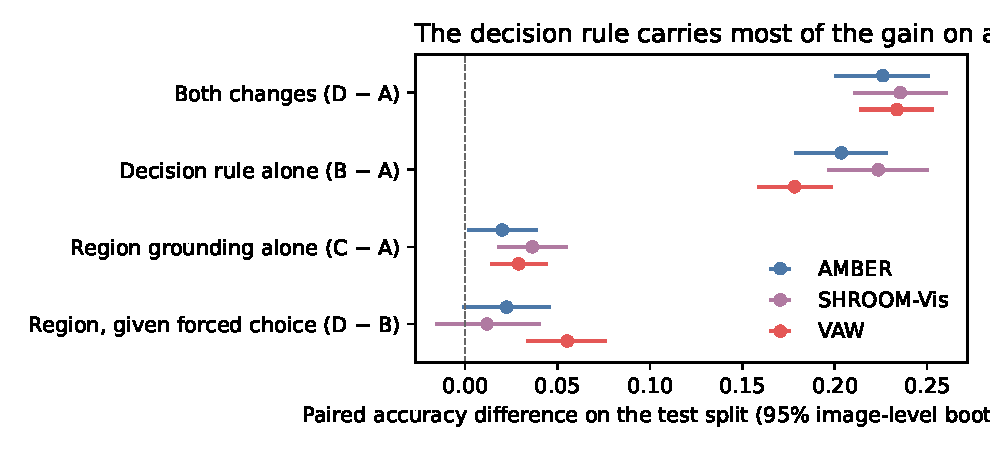
\includegraphics[width=0.92\textwidth]{figures/fig_attribution.pdf}
\caption{Attribution on the three test splits. Points are paired accuracy differences and bars are 95\% image-level bootstrap intervals. In every dataset the decision rule alone (B$-$A) accounts for most of the combined effect (D$-$A), while region grounding (C$-$A, D$-$B) contributes a smaller amount.}
\label{fig:attrib}
\end{figure}

\subsection{Removing the threshold versus calibrating it}\label{sec:calib}
The remedy that prior work offers for threshold failure is calibration~\cite{zhang2026visor,zhao2021calibrate}: if the boundary is in the wrong place, move it. Table~\ref{tab:calib} and Fig.~\ref{fig:calib} test this on the same scorer, regions and data. Two calibrators are fitted on development data: VISOR-style null-image correction (Cal-null, Eq.~\ref{eq:calnull}) and per-word thresholds (Cal-word). Two image-blind references show what can be achieved without the image. On VAW all four were declared before the test split was read. On AMBER and SHROOM-Vis they are post-hoc baselines computed from the existing logs.

\textbf{Null-image calibration does not help a contrastive scorer.} On all three datasets the development fit selects $\gamma\le 0.10$ (VAW: $\gamma=\VAWgammaA$ on both the whole image and the region), and Cal-null is within $\pm0.0013$ of the uncalibrated threshold on the test splits. This is consistent with Proposition~\ref{prop:offset}. The null-image prior $s(I_{\varnothing},a)$ does not depend on the image, so it can remove a word-level offset but not the image-level offset $c(R,o)$ that produces same-answer errors. It is also consistent with VISOR's own finding that the null-image prior is a weak predictor of false positives~\cite{zhang2026visor}. FC-null, a forced choice on the grey image, scores between 0.47 and 0.57, and cell D exceeds it by $+0.24$ to $+0.33$ (Table~\ref{tab:calib}). The scorer's text-only preference between the two words therefore explains little of forced choice's advantage.

\textbf{Per-word thresholds help, but largely by learning the word.} Cal-word is the strongest calibrator. On AMBER, whose attribute vocabulary is small and highly repetitive, it comes within $+0.0225$ $[-0.0075,+0.0528]$ of cell D. However, an image-blind WordPrior that never opens an image and only memorises which words tend to be the true attribute reaches 0.7592 there. Cal-word's margin over that image-blind prior is only $+0.0195$. On SHROOM-Vis, whose vocabulary is wider, the gap to forced choice reopens to $+0.1204$. On VAW, per-word thresholds fitted on development data do not transfer at all: Cal-word is $-0.0253$ below the \emph{uncalibrated} region threshold on test, the image-blind WordPrior falls to \VAWtestAccWordPrior, and cell D exceeds Cal-word by \VAWtestDminusCalWordC{} \VAWtestDminusCalWordCCI. Per-word calibration can move the threshold to a better place, but where it succeeds it does so partly by encoding the label distribution of the benchmark's vocabulary. That knowledge must be fitted per word on labelled data, and it transfers only as far as the label distribution does. Forced choice needs no labelled data and has no parameter.

\begin{table}[!htbp]
\centering
\caption{Calibrating the threshold versus removing it (test splits; same scorer, regions and questions). Acc: accuracy; FPR: share of false claims accepted. Calibration parameters are fitted on development data. On AMBER and SHROOM-Vis the calibrators and image-blind cells are post-hoc baselines; on VAW they were declared in advance.}
\label{tab:calib}
\small
\setlength{\tabcolsep}{4pt}
\begin{tabular}{lcccccc}
\toprule
 & \multicolumn{2}{c}{\textbf{AMBER}} & \multicolumn{2}{c}{\textbf{SHROOM-Vis}} & \multicolumn{2}{c}{\textbf{VAW}} \\
\cmidrule(lr){2-3}\cmidrule(lr){4-5}\cmidrule(lr){6-7}
Cell & Acc & FPR & Acc & FPR & Acc & FPR \\
\midrule
\tabinput{tables/calib_cells.tex}
\bottomrule
\end{tabular}\\[6pt]
\resizebox{\textwidth}{!}{%
\begin{tabular}{lcccccc}
\toprule
Contrast (AMBER $|$ SHROOM-Vis $|$ VAW) & $\Delta$ & 95\% CI & $\Delta$ & 95\% CI & $\Delta$ & 95\% CI \\
\midrule
\tabinput{tables/calib_contrasts.tex}
\bottomrule
\end{tabular}}
\end{table}

\begin{figure}[!htbp]
\centering
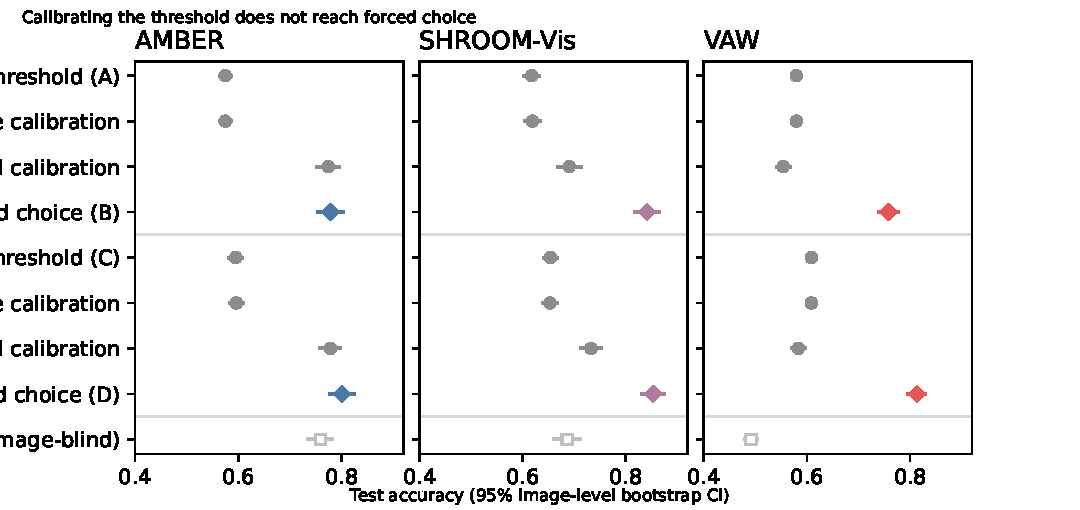
\includegraphics[width=\textwidth]{figures/fig_calibration.pdf}
\caption{Calibration baselines and forced choice on the same scorer (test splits, 95\% image-level bootstrap intervals). Diamonds: forced choice; circles: threshold and calibrated thresholds; open square: an image-blind word prior fitted on development labels.}
\label{fig:calib}
\end{figure}

\subsection{Why thresholding fails: pair-level analysis}\label{sec:mechanism}
Proposition~\ref{prop:offset} predicts that threshold errors are dominated by pairs whose two questions get the \emph{same} answer, rather than by pairs whose order is reversed. Table~\ref{tab:pairs} and Fig.~\ref{fig:pairs} classify every test pair. Under AMBER's baseline A, 666 of 845 pairs (78.8\%) get the same answer for both attributes and only 26 (3.1\%) are reversed. The same scores used as a forced choice (cell B) rank the true attribute first in 658 pairs (77.9\%). The scorer already separates the attributes in most pairs. What fails is the absolute threshold, because score levels shift from image to image: on the whole image, the two attribute scores of an AMBER frisbee pair are $(+0.42,-0.80)$ and those of a hydrant pair are $(-8.35,-7.90)$, about 8 logits apart (Fig.~\ref{fig:example}). The pattern repeats on SHROOM-Vis and VAW. Region grounding mostly \emph{moves} threshold errors between the both-yes and both-no columns, because crops shift the whole score distribution. It changes the share of correctly ordered pairs much less, so it helps a threshold slightly and a forced choice hardly at all.

\begin{table}[!htbp]
\centering
\caption{Outcome of every test pair. Correct: $a^{+}$ \yes, $a^{-}$ \no. Both-yes / both-no: the same answer to both questions (one error). Reversed: two errors. Forced-choice cells cannot produce same-answer outcomes.}
\label{tab:pairs}
\small
\begin{tabular}{llrrrrr}
\toprule
Dataset & Cell & Correct & Both-yes & Both-no & Reversed & Pairs \\
\midrule
\tabinput{tables/pairs.tex}
\bottomrule
\end{tabular}
\end{table}

\begin{figure}[!htbp]
\centering
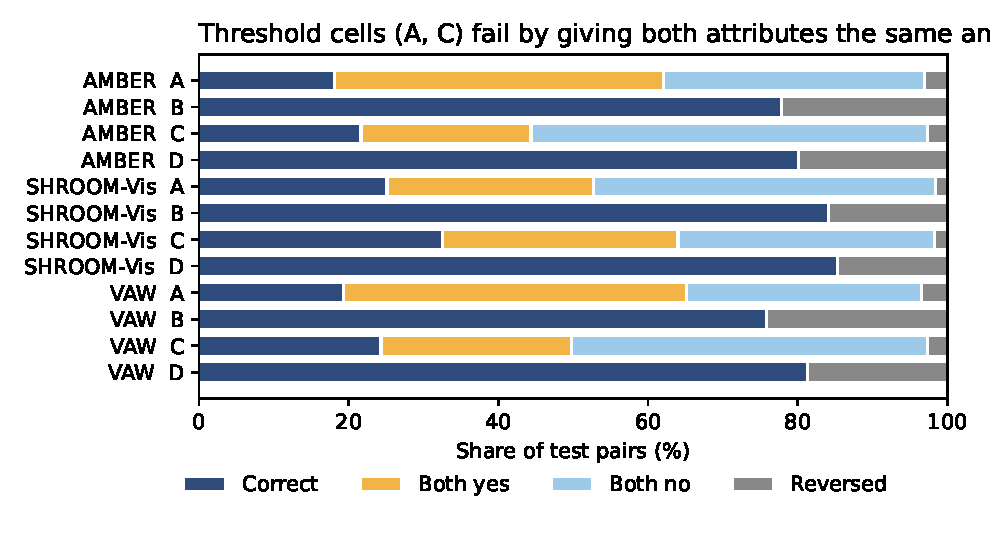
\includegraphics[width=0.92\textwidth]{figures/fig_pairs.pdf}
\caption{Pair outcomes on the three test splits. Threshold cells (A, C) fail mostly by giving the same answer to both attributes. Forced-choice cells (B, D) can only fail by reversing the order.}
\label{fig:pairs}
\end{figure}

\begin{figure}[!htbp]
\centering
\begin{subfigure}[t]{0.49\textwidth}
\centering
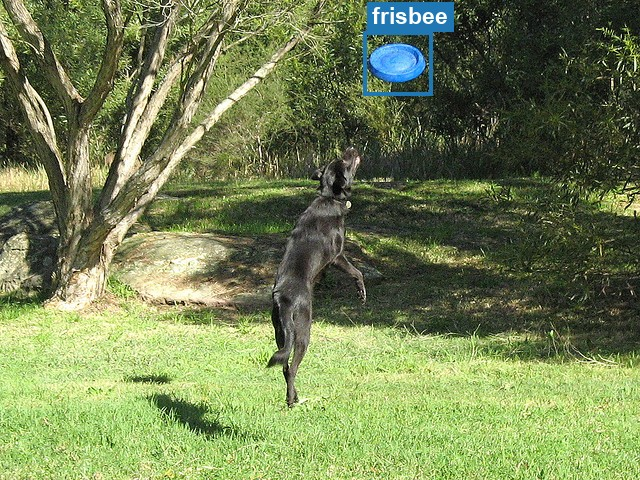
\includegraphics[height=3.0cm]{figures/amber188_boxes.jpg}\hspace{3pt}%
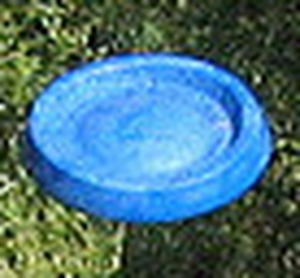
\includegraphics[height=3.0cm]{figures/amber188_crop_frisbee.jpg}
\caption{\texttt{AMBER\_188}: frisbee, blue (\yes) vs.\ black (\no)}
\end{subfigure}\hfill
\begin{subfigure}[t]{0.49\textwidth}
\centering
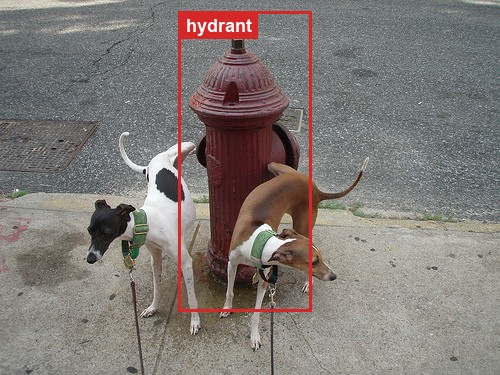
\includegraphics[height=3.0cm]{figures/amber75_boxes.jpg}\hspace{3pt}%
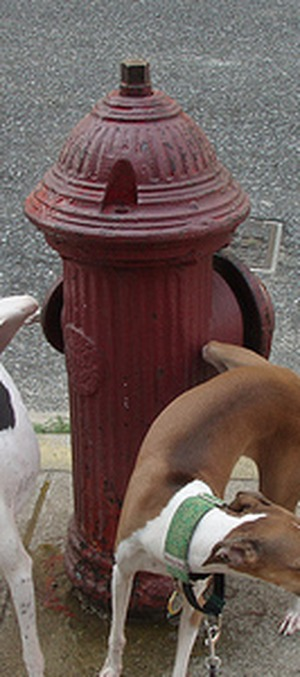
\includegraphics[height=3.0cm]{figures/amber75_crop_hydrant.jpg}
\caption{\texttt{AMBER\_75}: hydrant, red (\yes) vs.\ white (\no)}
\end{subfigure}\\[6pt]
\small
\begin{tabular}{lcccc}
\toprule
 & \multicolumn{2}{c}{Frisbee (black, blue)} & \multicolumn{2}{c}{Hydrant (red, white)} \\
\cmidrule(lr){2-3}\cmidrule(lr){4-5}
 & Logits & Outcome & Logits & Outcome \\
\midrule
Whole image, A ($\tau{=}-11.03$) & $(+0.42,\,-0.80)$ & both-yes & $(-8.35,\,-7.90)$ & both-yes \\
Whole image, B & & reversed & & reversed \\
Region, C ($\tau{=}-5.09$) & $(-5.55,\,+1.83)$ & correct & $(-2.58,\,-6.00)$ & correct \\
Region, D (proposed) & & correct & & correct \\
\bottomrule
\end{tabular}
\caption{Two AMBER test pairs, taken from the test logs. In each panel the left image shows the whole frame with the OWLv2 box and the right image the M3 crop. SigLIP logits are listed in alphabetical candidate order. On the whole image both scores clear the threshold, giving two \yes{} answers, and the forced choice prefers the wrong colour. The two images' score levels lie about 8 logits apart, which no single threshold can accommodate. These pairs were selected to show cases where the region matters; in the typical pair it does not (Table~\ref{tab:attrib}).}
\label{fig:example}
\end{figure}

\subsection{How much does grounding itself contribute? An oracle arm on VAW}\label{sec:oracle}
Region grounding could look small because grounding matters little, or because OWLv2 sometimes boxes the wrong instance. VAW annotates the instance each label refers to, so the oracle cells C$^{\ast}$ and D$^{\ast}$ can crop to the human box instead (Table~\ref{tab:oracle}). Detector error is real: under forced choice the oracle box adds \VAWtestDstarminusD{} \VAWtestDstarminusDCI{} over the detector box (D$^{\ast}$ reaches \VAWtestAccDstar), and under a threshold the oracle region gains \VAWtestCstarminusA{} over the whole image against \VAWtestCminusA{} for the detector region. But even perfect localisation does not make grounding rival the decision rule. With the oracle box, the decision rule still adds \VAWtestDstarminusCstar{} \VAWtestDstarminusCstarCI{} (D$^{\ast}-$C$^{\ast}$), about four times the oracle grounding effect under a threshold.

\begin{table}[!htbp]
\centering
\caption{Oracle grounding on VAW (test, 1{,}500 images). C$^{\ast}$/D$^{\ast}$ crop to the human-annotated instance box with the same padding as the detector crop.}
\label{tab:oracle}
\small
\begin{tabular}{lcc}
\toprule
Contrast & $\Delta$ & 95\% CI \\
\midrule
\tabinput{tables/vaw_oracle.tex}
\bottomrule
\end{tabular}
\end{table}

\subsection{Does the effect survive a different scorer? A generative-VLM check}\label{sec:vlm}
The factorial design holds the scorer fixed by construction, so the decision-rule effect could in principle be a property of SigLIP. We therefore repeated the decision-rule comparison with a scorer of a different class: a generative multimodal LLM (\texttt{\VLMmodel}) answering in natural language at temperature 0, probed exactly as VISOR probes its VLMs. VLM-threshold asks each question alone (``Is the \{object\} \{attribute\} in this image? Answer only yes or no''), so the model's own internal boundary plays the role of $\tau$. VLM-FC asks which of the two candidates, in alphabetical order, better describes the object. VLM-prior repeats the independent questions over a uniform grey image, the discrete analogue of VISOR's $\delta_{\mathrm{prior}}$. Table~\ref{tab:vlm} reports the result.

\textbf{Scope.} This check is smaller than planned and covers \emph{colour attributes only}: \VLMpairs{} pairs, \VLMquestions{} questions, on the VAW test split. The run was stopped part-way by an API budget limit of our execution environment, and because requests were issued in the frozen pair order, which is grouped by type, the completed calls form a colour-only prefix. \VLMdropped{} replies were unparseable and excluded, most of them in the grey-image arm, where the model declines to answer rather than guess. Token log-probabilities are not exposed by this API, so $\delta_{\mathrm{vis}}$ cannot be formed and \textbf{no calibration arm is possible for this scorer}: the comparison of calibration with forced choice in Section~\ref{sec:calib} remains a SigLIP result.

\textbf{The mechanism generalises; the magnitude shrinks.} Forced choice improves on independent probing by \VLMfcMinusThr{} \VLMfcMinusThrCI{} (\VLMaccThr{} to \VLMaccFC). The interval excludes zero, but only just, and the effect is about a quarter of the \VAWtestBminusA{} that the same contrast produces with SigLIP on the full VAW test split. The pair-level signature is nevertheless the same one Proposition~\ref{prop:offset} predicts: under independent probing \VLMpairSame{} of pairs receive the same answer to both questions, while only \VLMpairRev{} are reversed, so same-answer errors again dominate and forced choice converts most of them (\VLMpairCorrect{} to \VLMfcCorrect{} of pairs correct). What differs is the size of the problem to begin with. This VLM is not strongly yes-biased on colour: its Yes-ratio is \VLMyesThr{} and its false-positive rate \VLMfprThr, where the whole-image threshold cell on the same dataset accepts about half of all false colour claims. A model that effectively sets its own boundary per image has less of the miscalibration that forced choice removes. The grey-image arm confirms the model is reading the image rather than the words: it answers \yes{} to only \VLMyesPrior{} of questions without visual evidence, and VLM-threshold beats VLM-prior by \VLMthrMinusPrior{} \VLMthrMinusPriorCI.

\textbf{What this does and does not license.} It supports the claim that the pair-level failure mode is a property of \emph{independent absolute verification}, not of one scorer. It does not license a claim that forced choice yields a large gain for every scorer: on colour, for a strong generative VLM, the gain is small. The practical reading is that the weaker and the less calibrated the verifier, the more the decision rule matters, which is also why it matters most for the cheap, language-model-free verifier this paper is built on.

\begin{table}[!htbp]
\centering
\caption{Generative-VLM check on VAW (\texttt{\VLMmodel}, temperature 0; \VLMpairs{} colour pairs, \VLMquestions{} questions, \VLMpairs{} images). YR: Yes-ratio. Pair outcomes as in Table~\ref{tab:pairs}; a forced choice cannot produce same-answer outcomes. Accuracy intervals are 95\% image-level bootstrap intervals. Colour only, and no calibration arm is possible for this scorer (see text).}
\label{tab:vlm}
\small
\setlength{\tabcolsep}{4pt}
\resizebox{\textwidth}{!}{%
\begin{tabular}{lccccrrrr}
\toprule
Arm & Acc & 95\% CI & YR & FPR & Correct & Both-yes & Both-no & Reversed \\
\midrule
\tabinput{tables/vlm.tex}
\bottomrule
\end{tabular}}
\end{table}

\subsection{Controls}\label{sec:controlsres}
\textbf{The free answer prior does not explain forced choice.} Base-rate-matched thresholds (A$'$) gain almost nothing over A, and forced choice net of that prior (B$-$A$'$) remains large on every dataset (Table~\ref{tab:controls}). A$'$ imposes a \emph{global} base rate, whereas forced choice imposes a \emph{per-pair} constraint. A threshold rule cannot use the per-pair constraint without comparing the candidates, which is exactly what forced choice does.
\textbf{The dataset's competitor is not required.} D-ext answers each question alone against a generic antonym from a map committed before any D-ext result existed and never modified. It keeps most of the gain over A on its covered subset (Table~\ref{tab:controls}). Its coverage is 94.0\% of questions on AMBER, 84.3\% on SHROOM-Vis and \VAWtestDextCoverage{} on VAW, where the most frequent unmapped words are materials with no natural opposite (\emph{metal}, \emph{brick}, \emph{stone}, \emph{glass}). Forced choice requires a competing hypothesis, and where none exists the method does not apply.

\begin{table}[!htbp]
\centering
\caption{Controls (test splits). A$'$: base-rate-matched threshold. D-ext: each question decided alone against a pre-registered antonym; compared with A on the covered subset.}
\label{tab:controls}
\small
\begin{tabular}{lccc}
\toprule
Dataset & A$'$ accuracy & B $-$ A$'$ [95\% CI] & D-ext $-$ A (covered) [95\% CI] \\
\midrule
\tabinput{tables/controls.tex}
\bottomrule
\end{tabular}
\end{table}

\textbf{Benchmark artifacts in AMBER.}\label{sec:artifacts} Three construction artifacts let an image-blind strategy score 1.0000 on AMBER. (i) In all 2{,}774 attribute pairs the true attribute holds the lower question id. (ii) All 4{,}924 existence questions have gold \no. (iii) Relation gold is constant within each relation sub-type. We report these rather than exploit them. No cell reads question ids: under permuted ids the position-only baseline falls to 0.41 while cells A and D produce bit-identical output. The state and action questions used here are exactly balanced. SHROOM-Vis and VAW assign ids within a pair by a seeded coin flip, so position-only scores 0.5503 on the SHROOM-Vis test split.

\subsection{Comparison with VISOR on VAW}\label{sec:visor}
Table~\ref{tab:visor} reports, per attribute type, the metrics VISOR uses (accuracy, F1 with \yes{} as positive, Yes-ratio and FPR) for our cells, next to the numbers VISOR reports for its baseline and its routed method on three VLMs~\cite{zhang2026visor}. \textbf{The two halves of the table are not like-for-like}, and we do not claim to outperform VISOR. VISOR probes 3--7B VLMs on its own VAW sample, which is unbalanced (for example 1{,}302 positive and 1{,}690 negative colour samples), and its material row uses trained per-word adapters. Our cells use a 0.2B contrastive scorer on balanced pairs drawn from the same VAW types. The comparison that \emph{is} controlled is the upper half of the table, where calibration and forced choice share one scorer. Two observations follow. First, VISOR's qualitative diagnosis also holds for a contrastive scorer: the threshold cells accept many false attributes (whole-image FPR 45--60\%). Second, neither calibrator lowers FPR consistently on this scorer. Cal-null leaves it unchanged ($\gamma=0$), and Cal-word raises it for colour and material while lowering it for state on the whole image. Third, removing the threshold lowers FPR for every attribute type (to 15--23\% in cell D), without per-type routing and without training.

\begin{table}[!htbp]
\centering
\caption{VAW per attribute type, with VISOR's metrics (\%). Upper block: this work, test split, balanced pairs, SigLIP scorer. Lower block: quoted from VISOR, Table~I~\cite{zhang2026visor}, on VISOR's own (unbalanced) VAW sample with VLM scorers; ``VISOR'' is its routed method (Calib for colour/state, trained Adapt for material). The two blocks differ in scorer, sample and class balance and are \emph{not} directly comparable.}
\label{tab:visor}
\scriptsize
\setlength{\tabcolsep}{3pt}
\begin{tabular}{lcccccccccccc}
\toprule
 & \multicolumn{4}{c}{\textbf{Color}} & \multicolumn{4}{c}{\textbf{Material}} & \multicolumn{4}{c}{\textbf{State}} \\
\cmidrule(lr){2-5}\cmidrule(lr){6-9}\cmidrule(lr){10-13}
 & Acc & F1 & YR & FPR & Acc & F1 & YR & FPR & Acc & F1 & YR & FPR \\
\midrule
\multicolumn{13}{l}{\emph{This work (SigLIP-base, 0.2B; OWLv2 regions; balanced pairs)}} \\
\tabinput{tables/vaw_types.tex}
\midrule
\multicolumn{13}{l}{\emph{Quoted from VISOR~\cite{zhang2026visor} (VLM yes/no probing; VISOR's sample)}} \\
Qwen2.5-VL-3B baseline & 73.9 & 73.7 & 55.6 & 33.8 & 79.0 & 73.0 & 37.9 & 15.7 & 74.1 & 71.0 & 46.6 & 25.9 \\
Qwen2.5-VL-3B + VISOR & 75.1 & 71.4 & 43.7 & 22.2 & 79.9 & 73.9 & 37.0 & 14.2 & 75.5 & 70.4 & 40.0 & 19.0 \\
InternVL3.5-4B baseline & 75.2 & 74.7 & 54.4 & 31.6 & 78.8 & 74.2 & 42.3 & 19.5 & 71.2 & 66.7 & 43.5 & 25.7 \\
InternVL3.5-4B + VISOR & 76.9 & 71.7 & 37.8 & 15.4 & 80.3 & 75.9 & 41.7 & 17.8 & 72.5 & 65.8 & 37.7 & 19.6 \\
LLaVA-1.5-7B baseline & 65.8 & 67.8 & 62.6 & 47.2 & 74.7 & 70.5 & 45.7 & 25.8 & 70.1 & 67.8 & 50.1 & 32.5 \\
LLaVA-1.5-7B + VISOR & 68.9 & 65.2 & 46.1 & 29.8 & 76.2 & 72.3 & 45.7 & 24.5 & 70.1 & 67.8 & 50.1 & 32.5 \\
\bottomrule
\end{tabular}
\end{table}

\subsection{Comparison with other detectors and evaluation protocols}\label{sec:sota}
\textbf{Claim-level protocol of UNIHD and OmniHallu.} Table~\ref{tab:hnh} reports precision, recall and F1 separately for hallucinated and non-hallucinated claims, and their macro average, following~\cite{chen2024unihd,yang2026omnihallu}. The threshold cells are lopsided. On AMBER, region cropping under a threshold (C) raises hallucinated-claim recall to 74.7\% but lowers non-hallucinated recall to 44.4\%, which is again a symptom of a misplaced criterion. The forced-choice cells are balanced by construction. These numbers are not comparable with OmniHallu's or UNIHD's own results, which are measured on different benchmarks with open-ended claims.

\begin{table}[!htbp]
\centering
\caption{Claim-level metrics in the protocol of UNIHD/OmniHallu~\cite{chen2024unihd,yang2026omnihallu} (test splits, \%). H: hallucinated claims (gold \no); NH: non-hallucinated claims (gold \yes).}
\label{tab:hnh}
\small
\setlength{\tabcolsep}{4pt}
\begin{tabular}{llrrrrrrrr}
\toprule
 & & \multicolumn{3}{c}{Hallucinated} & \multicolumn{3}{c}{Non-hallucinated} & \multicolumn{2}{c}{Overall} \\
\cmidrule(lr){3-5}\cmidrule(lr){6-8}\cmidrule(lr){9-10}
Dataset & Cell & P & R & F1 & P & R & F1 & Acc & Mac.F1 \\
\midrule
\tabinput{tables/hnh.tex}
\bottomrule
\end{tabular}
\end{table}

\textbf{VLMs answering AMBER's attribute questions.} AMBER reports attribute F1 for VLMs answering its questions directly~\cite{wang2023amber}: mPLUG-Owl 22.9, MiniGPT-4 43.7, LLaVA 48.6, CogVLM 57.4, LLaVA-1.5 64.6, mPLUG-Owl2 72.4, InstructBLIP 76.3, Qwen-VL 81.4 and GPT-4V 82.2. Cell D reaches 80.1 on the test split (80.5 over all 5{,}548 state and action questions, as it has no fitted parameter), and the threshold cell A built from the same models reaches 59.4. The comparison is indicative only. AMBER's figures include number questions, which we exclude, and the VLMs answer each question alone. D-ext, which also answers alone, reaches an F1 of 77.0.

\textbf{SHROOM-Visions 2026.} The top English systems of SHROOM-Visions fine-tune 8B-scale Qwen VLMs with LoRA or combine them with MLLM judges, and they score character-level spans by correlation and IoU~\cite{vazquez2026shroomvisions}. SpanCalib-VLM fuses a span tagger with a fine-tuned 4B VLM through calibrated probabilities~\cite{abebe2026spancalib}. Their task, labels and metric differ from ours, so no numerical comparison is valid. The approaches are complementary: a span-level system could locate the attribute claims in a free-form response, and a verifier like ours could then check each one cheaply.

\subsection{Computational cost}\label{sec:cost}
The verifier has 358.1M parameters (OWLv2 155.0M, SigLIP 203.2M), uses no language model and no paid API, and peaked at 1.65\,GiB of GPU memory on a 4\,GB RTX~3050 Laptop GPU. With detections cached, scoring an attribute question takes about 32\,ms. Cells A and D cost the same, because forced choice scores the same two prompts as the threshold rule. On VAW, the same hardware processed 1{,}500 pairs (detection and scoring of three regions plus the null image) in about 40 minutes per split. For context, OmniHallu reports 5--8 API calls and about \$0.12 per sample for its full pipeline~\cite{yang2026omnihallu}, and VBackChecker uses a 7B grounding LLM~\cite{guo2026vbackchecker}.

%% ---------------------------------------------------------------------
\section{Discussion}\label{sec:discussion}
%% ---------------------------------------------------------------------
\textbf{What the factorial design shows.} With the scorer, prompts and data fixed, the decision rule is the dominant factor in attribute hallucination detection on three datasets that differ in source, annotation and vocabulary. Region grounding is real and positive. Its largest effect given forced choice is on VAW's cluttered scenes, where it is also limited by detector error (Section~\ref{sec:oracle}), but it is several times smaller than the decision-rule effect on every dataset. These are the measurements that end-to-end evaluation of grounding-centred detectors~\cite{guo2026vbackchecker,song2026countervhd} cannot provide, because grounding and the decision are changed together there.

\textbf{Relation to calibration.} VISOR~\cite{zhang2026visor} diagnosed many attribute errors as threshold-placement errors and calibrated the threshold. Our pair-level analysis agrees with the diagnosis and adds a reason why calibration has limits. The offset that defeats a fixed threshold varies with the image (Proposition~\ref{prop:offset}), whereas a calibrator is fitted per word or per prior. The best calibrator we tested recovers much of its gain by learning the benchmark's word-level label distribution, which an image-blind baseline reproduces. Forced choice cancels the image-level offset by construction. The two remedies are not exclusive: VISOR's visual margin $\delta_{\mathrm{vis}}$ could itself be used in a forced choice, $\delta_{\mathrm{vis}}(a^{+})$ against $\delta_{\mathrm{vis}}(a^{-})$, which we leave to future work. The generative-VLM check in Section~\ref{sec:vlm} points the same way: the better calibrated the verifier already is, the less the decision rule has to fix.

\textbf{Where the method fails.} The remaining errors of cell D are reversed pairs, in which SigLIP's attribute--object binding is wrong even on the region. No decision rule can repair these, and a stronger scorer is needed. Forced choice also needs a competing hypothesis. Where a dataset does not supply one, a generic antonym map recovers most of the gain but covers only part of the vocabulary.

%% ---------------------------------------------------------------------
\section{Limitations and Threats to Validity}\label{sec:threats}
%% ---------------------------------------------------------------------
\begin{itemize}[leftmargin=*]
\item \textbf{Scorer coverage.} The factorial design holds SigLIP fixed by intention. The generative-VLM check (Section~\ref{sec:vlm}) extends it to one other scorer class, but only on colour attributes, on \VLMpairs{} pairs, and without access to token log-probabilities, so VISOR-Calib could not be reproduced for that scorer and a forced choice taken directly on $\delta_{\mathrm{vis}}$ remains untested. The material and state types, the region factor and open-weight VLM scorers are left to future work.
\item \textbf{Competitor availability.} Forced choice requires a competing attribute. On all three datasets it comes from the data (benchmark pair, frozen policy or human negative label). D-ext shows that a generic antonym retains most of the gain, but its coverage is incomplete, especially for materials and actions.
\item \textbf{Post-hoc baselines.} The calibration baselines and image-blind cells were added to AMBER and SHROOM-Vis after their test splits had been opened. They are baselines, not changes to the method, and on VAW they were declared in advance.
\item \textbf{Silver labels.} SHROOM-Vis was annotated by a VLM, under a frozen policy and without human verification. It is easier than AMBER, so only within-dataset contrasts are interpreted.
\item \textbf{VAW construction.} VAW is not exhaustively annotated, so a ``negative'' attribute can occasionally be visually plausible (VISOR documents this for \emph{steel}). Our unique-name filter reduces, but does not remove, referential ambiguity. Development pairs for the rarer types were completed from VAW's training split. The VAW software environment (torch 2.14.1) differed from that of AMBER and SHROOM-Vis (torch 2.6.0), although the model revisions, configuration and Transformers version were the same.
\item \textbf{Scope.} The study covers English templated claims and zero-shot models. It does not evaluate end-to-end detection on free-form captions, where errors in claim extraction would add to verification errors, and confidence calibration is not a claim of this work.
\end{itemize}

%% ---------------------------------------------------------------------
\section{Conclusion}\label{sec:conclusion}
%% ---------------------------------------------------------------------
Prior work has shown that threshold-based attribute verification fails largely through threshold placement, and that calibration can move the threshold. This paper removes the dependence on that threshold instead: it replaces independent threshold-based verification with pairwise forced-choice verification. It then uses a controlled $2\times2$ factorial design, with the scorer, prompts and data held fixed, to separate the contribution of the decision rule from that of region grounding. On AMBER, SHROOM-Vis and VAW, the relative decision rule explains most of the observed gain. Region grounding contributes a smaller, real amount that does not come to rival the decision rule even with oracle boxes. Calibrated thresholds on the same scorer do not reach forced choice, and the best of them relies partly on a word-level label prior. A generative multimodal LLM probed the same way shows the same pair-level failure but a much smaller gain, which bounds the claim to verifiers whose decision boundary is not already well placed. Because the pair-level failure is specific (correct rankings, same answers), the practical recommendation is also specific: wherever a competing hypothesis is available, verify attribute claims by comparison rather than by threshold.

\section*{Data and Code Availability}
AMBER is redistributed under its Apache-2.0 licence. VAW annotations are available from the VAW repository and images from Visual Genome. SHROOM-Vis annotations, the frozen annotation policy, the VAW pair-construction script and protocol, all per-question logs, run manifests and the scripts that generate every table and figure in this paper are released with the code.

\section*{Conflict of Interest}
The authors declare no conflict of interest.

\bibliographystyle{unsrt}
\bibliography{references}

\appendix
\section{Evidence for the research-gap assessment}\label{app:evidence}
Table~\ref{tab:evidence} lists where, in each cited paper, the evidence for the entries of Table~\ref{tab:gap} is found.

\begin{table}[!htbp]
\centering
\caption{Evidence locations for Table~\ref{tab:gap}.}
\label{tab:evidence}
\footnotesize
\begin{tabularx}{\textwidth}{@{}l>{\raggedright\arraybackslash}X@{}}
\toprule
Work & What was checked, and where \\
\midrule
VISOR~\cite{zhang2026visor} & Threshold-placement diagnosis and calibrated rule $\mathbb{1}[\delta_{\mathrm{vis}}-\gamma\delta_{\mathrm{prior}}>0]$ (abstract; Sec.~III, ``Unified routing''). Each query ``Is the [object] [attribute]?'' is decided alone (Sec.~III--IV). No region annotations are used (Sec.~II). Low-margin signals are reported per sample and per word (Sec.~V; Tables~I, VI). \\
VBackChecker~\cite{guo2026vbackchecker} & A single [SEG]/[REJ] decision per sentence (Method). Ablation of the grounding loss and token weighting (Table~5). Negative/positive-accuracy imbalance of MLLM detectors (Table~3). \\
OmniHallu~\cite{yang2026omnihallu} & Expert majority voting and LLM aggregation (Sec.~5). UNIHD claim-level protocol (Table~3). Module ablation of claim decomposition and voting (Table~4). Calibration reward and ECE (Table~5). \\
Counterfactual grounding~\cite{song2026countervhd} & Factual and counterfactual confidences combined into an uncertainty $U_e$, decided by $U_e>\tau$ (Sec.~2). Threshold sensitivity (Fig.~3). \\
SpanCalib-VLM~\cite{abebe2026spancalib} & Union-calibrated fusion and calibration-centred evaluation (abstract; results table; limitations). \\
ARO / Winoground / SugarCrepe~\cite{yuksekgonul2023bow,thrush2022winoground,hsieh2023sugarcrepe} & Forced choice used as an \emph{evaluation} protocol for compositionality, not as a detector's decision rule. \\
\bottomrule
\end{tabularx}
\end{table}

\end{document}
